\section{Aufnahmen}
\begin{figure}
\centering
\label{fig:anfangssignal_ohne_rausch}
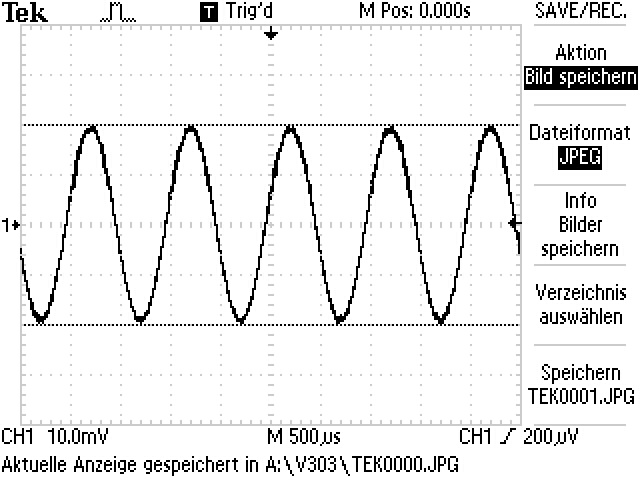
\includegraphics{aufnahmen(pdf)/eingangssignal.pdf}
\caption{Vom Funktionsgenerator erzeugte Sinusspannung}
\end{figure}
\begin{figure}
\centering
\label{fig:referenzsignal_ohne_rausch}
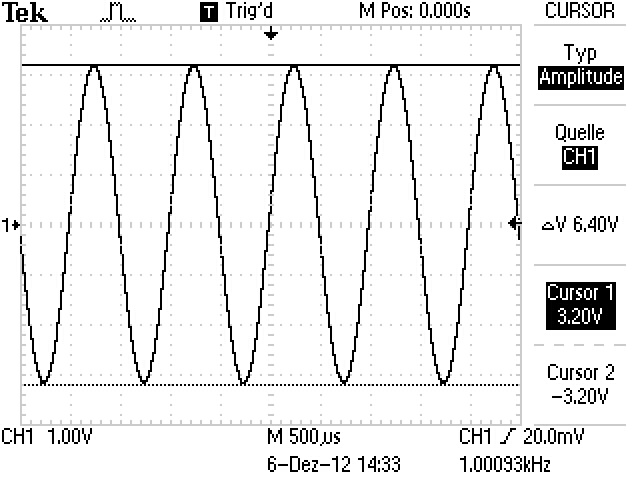
\includegraphics{aufnahmen(pdf)/referenzsignal.pdf}
\caption{Vom Funktionsgenerator erzeugtes Referenzsignal}
\end{figure}
\begin{figure}
\centering
\label{fig:phase_0_nicht_verrauscht}
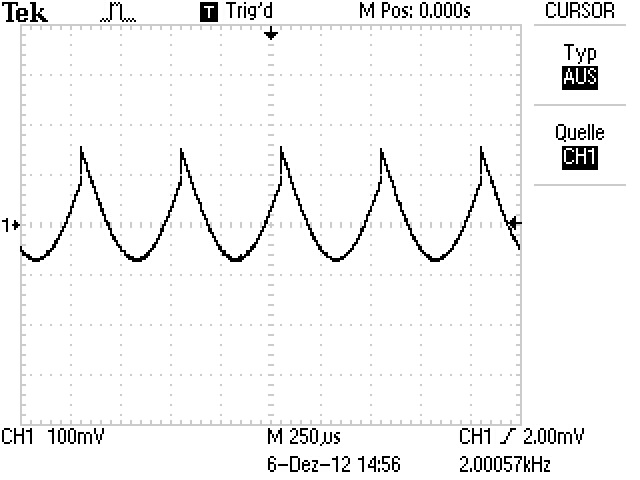
\includegraphics{aufnahmen(pdf)/phase_0_ohne_rauschen.pdf}
\caption{Nicht verrauschtes Mischsignal bei eingestellter Phasenverschiebung von \SI{0}{\degree}}
\end{figure}
\begin{figure}
\centering
\label{fig:phase_45_nicht_verrauscht}
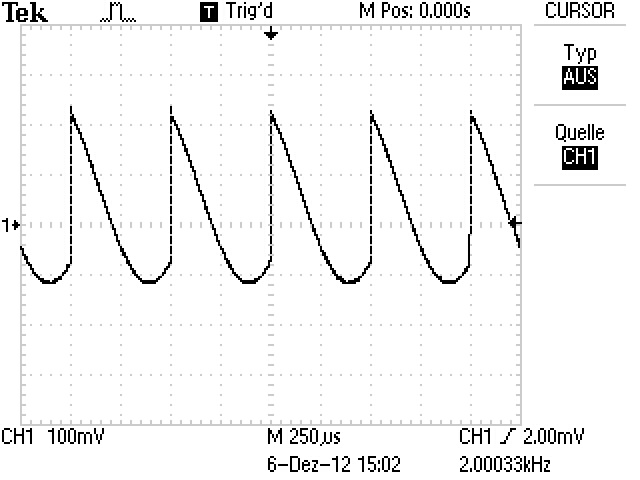
\includegraphics{aufnahmen(pdf)/phase_45_ohne_rauschen.pdf}
\caption{Nicht verrauschtes Mischsignal bei eingestellter Phasenverschiebung von \SI{45}{\degree}}
\end{figure}
\begin{figure}
\centering
\label{fig:phase_90_nicht_verrauscht}
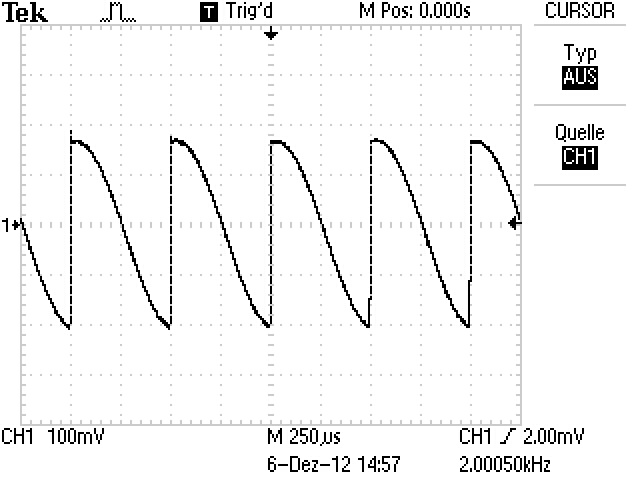
\includegraphics{aufnahmen(pdf)/phase_90_ohne_rauschen.pdf}
\caption{Nicht verrauschtes Mischsignal bei eingestellter Phasenverschiebung von \SI{90}{\degree}}
\end{figure}
\begin{figure}
\centering
\label{fig:phase_180_nicht_verrauscht}
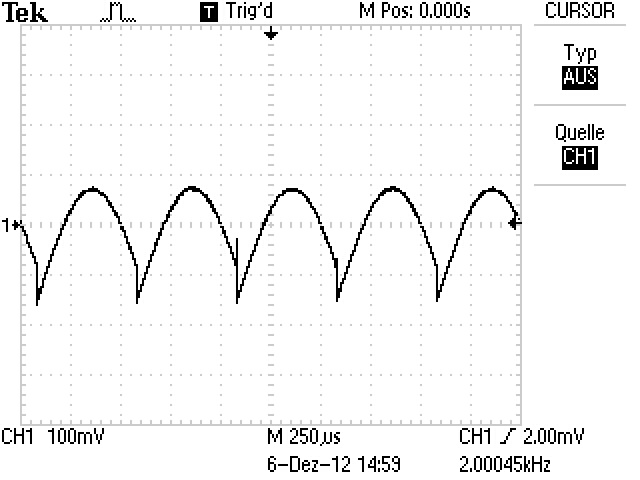
\includegraphics{aufnahmen(pdf)/phase_180_ohne_rauschen.pdf}
\caption{Nicht verrauschtes Mischsignal bei eingestellter Phasenverschiebung von \SI{180}{\degree}}
\end{figure}
\begin{figure}
\centering
\label{fig:phase_270_nicht_verrauscht}
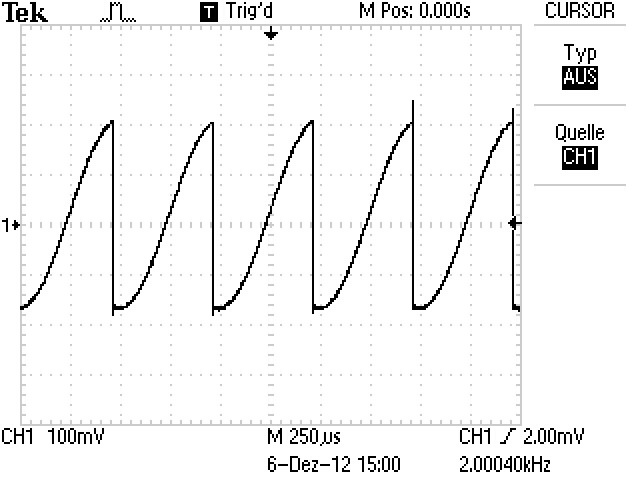
\includegraphics{aufnahmen(pdf)/phase_270_ohne_rauschen.pdf}
\caption{Nicht verrauschtes Mischsignal bei eingestellter Phasenverschiebung von \SI{270}{\degree}}
\end{figure}
\begin{figure}
\centering
\label{fig:gleichspannung_ohne_rausch}
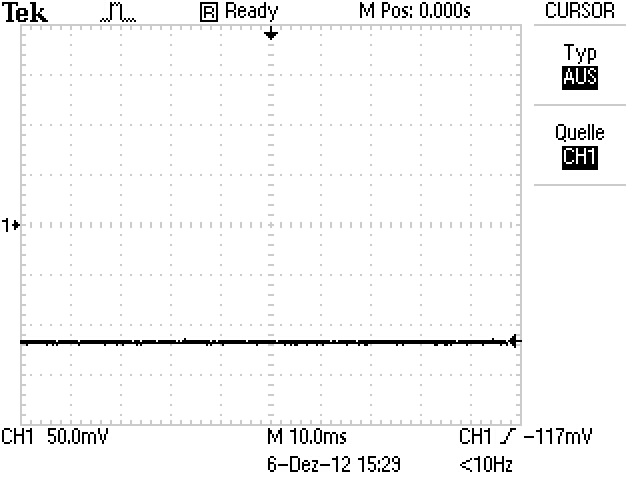
\includegraphics{aufnahmen(pdf)/gleichspannung_ohne_rauschen.pdf}
\caption{Ausgangssignal des Lock-In-Verstärkers bei nicht verrauschtem Eingangssignal}
\end{figure}
\begin{figure}
\centering
\label{fig:vollrausch}
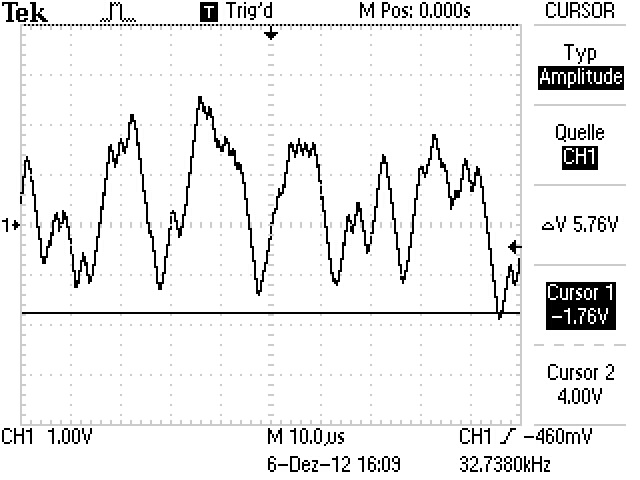
\includegraphics{aufnahmen(pdf)/vollrausch.pdf}
\caption{Verrauschtes Eingangssignal}
\end{figure}
\begin{figure}
\centering
\label{fig:bandrausch}
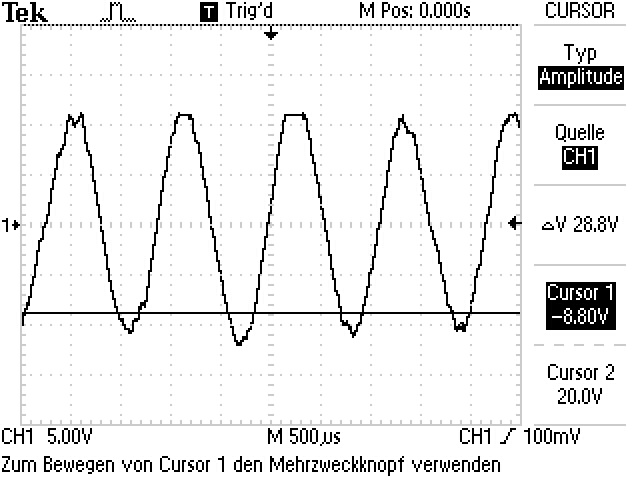
\includegraphics{aufnahmen(pdf)/bandrausch.pdf}
\caption{Form des verrauschten Signales nach Bandpassfilter}
\end{figure}
\begin{figure}
\centering
\label{fig:phase_0_verrauscht}
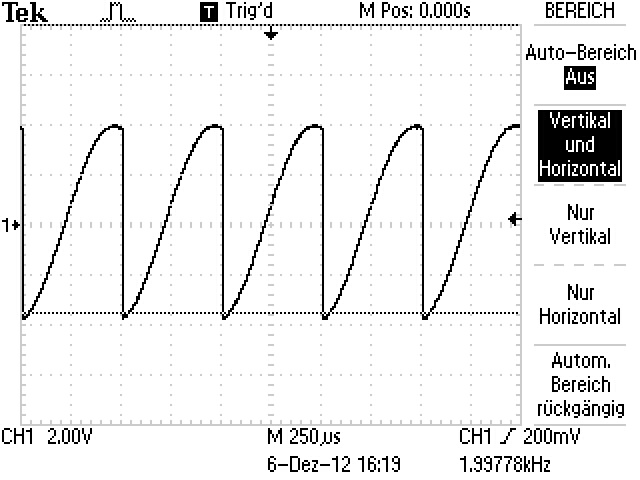
\includegraphics{aufnahmen(pdf)/phase_0_verrauscht.pdf}
\caption{Verrauschtes Mischsignal bei eingestellter Phasenverschiebung von \SI{0}{\degree}}
\end{figure}
\begin{figure}
\centering
\label{fig:phase_45_verrauscht}
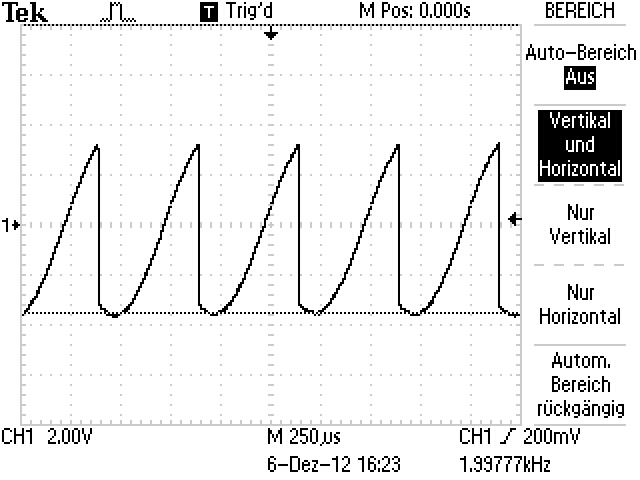
\includegraphics{aufnahmen(pdf)/phase_45_verrauscht.pdf}
\caption{Verrauschtes Mischsignal bei eingestellter Phasenverschiebung von \SI{45}{\degree}}
\end{figure}
\begin{figure}
\centering
\label{fig:phase_90_verrauscht}
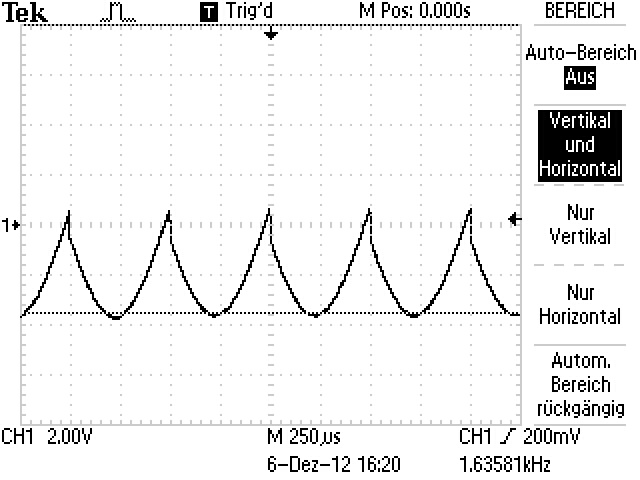
\includegraphics{aufnahmen(pdf)/phase_90_verrauscht.pdf}
\caption{Verrauschtes Mischsignal bei eingestellter Phasenverschiebung von \SI{90}{\degree}}
\end{figure}
\begin{figure}
\centering
\label{fig:phase_180_verrauscht}
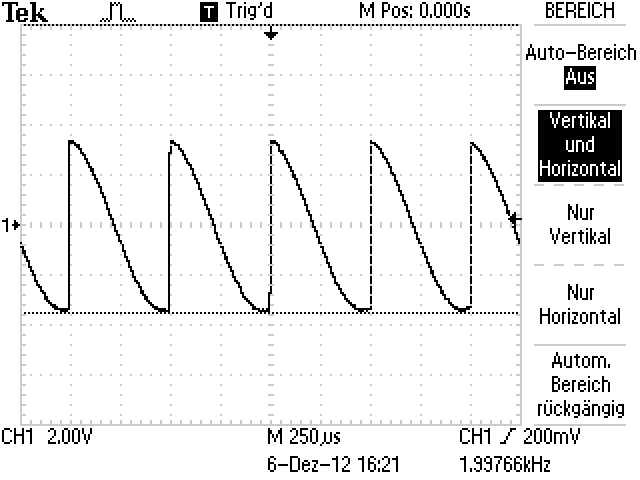
\includegraphics{aufnahmen(pdf)/phase_180_verrauscht.pdf}
\caption{Verrauschtes Mischsignal bei eingestellter Phasenverschiebung von \SI{180}{\degree}}
\end{figure}
\begin{figure}
\centering
\label{fig:phase_270_verrauscht}
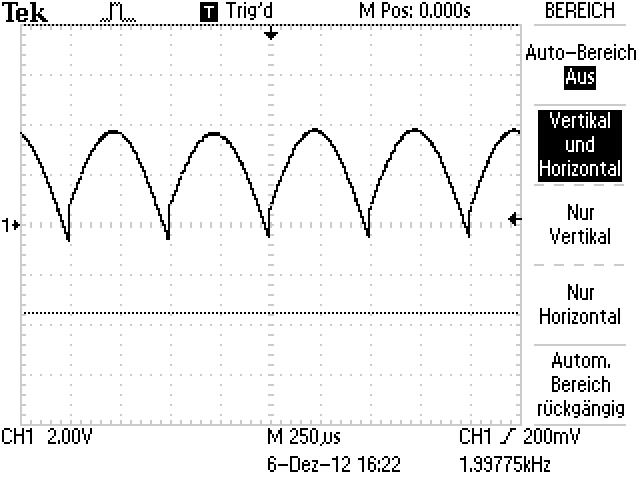
\includegraphics{aufnahmen(pdf)/phase_270_verrauscht.pdf}
\caption{Verrauschtes Mischsignal bei eingestellter Phasenverschiebung von \SI{270}{\degree}}
\end{figure}

